\begin{document}
\newcommand{\yhatone}{\bm\hat{\bm y}_1}
\newcommand{\yhattwo}{\bm\hat{\bm y}_2}
\newcommand{\yold}{\bm y_{\mathit{old}}}
In questo capitolo è descritta nel dettaglio l'architettura software sviluppata
per il progetto di locallizazione indoor, inclusa la rete neurale, le librerie
utilizzate, gli ambienti di sviluppo e gli strumenti che hanno coadiuvato il
testing e la sperimentazione del prototipo realizzato.
\section{TensorFlow}
%%%%%%%%%%%%%%%%%%%%%%%%%%%%%%%%%%%%%%%%%%%%%%%%%%%%%%%%%%%%%%%%%%%%%%%%%%%%%%%
\section{Keras}
%%%%%%%%%%%%%%%%%%%%%%%%%%%%%%%%%%%%%%%%%%%%%%%%%%%%%%%%%%%%%%%%%%%%%%%%%%%%%%%
\section{Google Colab}
%%%%%%%%%%%%%%%%%%%%%%%%%%%%%%%%%%%%%%%%%%%%%%%%%%%%%%%%%%%%%%%%%%%%%%%%%%%%%%%
\section{Weights \& Biases}
%%%%%%%%%%%%%%%%%%%%%%%%%%%%%%%%%%%%%%%%%%%%%%%%%%%%%%%%%%%%%%%%%%%%%%%%%%%%%%%
\section{Architettura della Rete Neurale}
\begin{figure}[!htp]
  % \makebox[\textwidth][c]{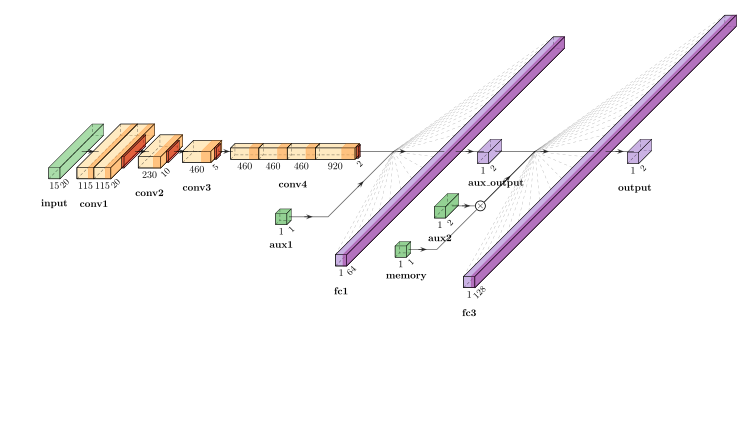
\includegraphics[width=1.0\textwidth]{./img/architettura.pdf}}%
  \makebox[\textwidth][c]{%
    \includetikz{0.75}{./img/architettura}%
  }%
  % 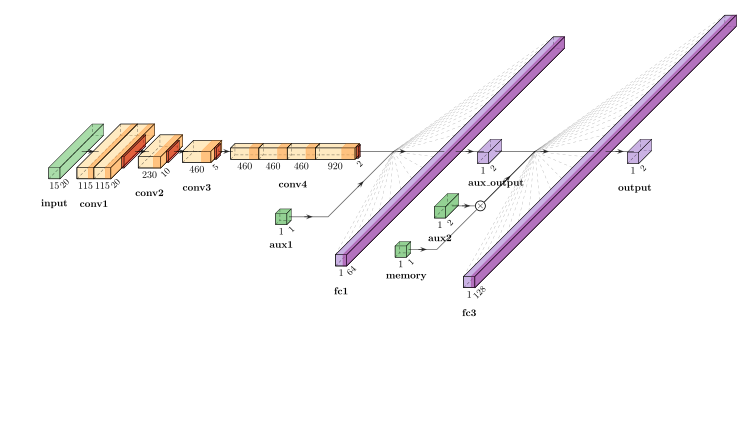
\includegraphics[width=1.3\textwidth]{./img/architettura.pdf}
  % \includetikz{0.8}{./img/architettura.tex}
  \caption{Architettura della rete neurale}%
  \label{fig:crynet}%
\end{figure}
La rete neurale sviluppata per il problema di localizzazione indoor è
illustrata schematicamente in Figura~\ref{fig:crynet}. Essa consiste in una
serie di blocchi convoluzionali seguiti da alcuni livelli di neuroni
completamente connessi. Il modello sfrutta, oltre ai segnali RSSI emessi dai
beacon, anche due input ausiliari che non sono processati dalla sezione
convoluzionale della rete.
\subsection{Input del Modello}
L'input principale del modello è composto da una serie temporale di valori RSSI
relativi ai segnali emessi da 15 beacon disposti lungo il perimetro
dell'edificio nel quale si sono svolte le sperimentazioni del prototipo. La
dimensione temporale dell'input può essere arbitrariamente lunga, poichè una
sua variazione determina solamente una differente dimensione dell'asse
temporale dell'output della CNN\@. La sezione convoluzionale della rete si
conclude infatti con un livello di pooling globale che consiste
nell'estrazione, per ogni feature map prodotta, della media aritmetica dei
valori di input lungo la dimensione del tempo. Come si vede in
Figura~\ref{fig:crynet}, infatti, la dimensione dell'output di tale livello è
sempre costante e risulta essere $920\times1$.

A completare l'input del modello sono il valore emesso dal sensore magnetico
dello smartphone e l'ultima posizione nota dell'utente all'interno
dell'edificio, indicati rispettivamente con \(\alpha\) e \( \yold \). Il
valore della bussola è utile per determinare l'orientamento della persona nello
spazio, rendendo la rete neurale capace di considerare le variazioni dei
segnali BLE dovuti all'assorbimento da parte del corpo dell'utilizzatore dello
smartphone. Il secondo input ausiliario è invece utilizzato per correggere
eventuali scostamenti rilevanti dell'output della CNN rispetto alla posizione
precedente dell'utente. Ci si aspetterebbe infatti che tale posizione non
variasse di molto in un lasso di tempo breve.

L'ultima posizione nota dell'utente viene pesata da un coefficiente, anche esso
input del modello, che in Figura~\ref{fig:crynet} è indicato con la lettera
greca \(\mu\). Tale valore, cui possiamo riferirci con il termine
\emph{coefficiente di memoria residua}, è compreso tra zero e uno, e determina
il peso che si vuole dare all'ipotesi di continuità della posizione dell'utente
nel tempo.  \(\mu = 0\) indica l'assenza di tale assunzione, con la conseguente
massima riduzione della correzione dell'output della CNN da parte dei livelli
successivi, mentre \(\mu = 1 \) associa il massimo peso su tale ipotesi. Il
coefficiente di memoria residua è esso stesso input del livello successivo
della rete, il quale riceve anche i valori dell'output ausiliario e di 
\(\mu \cdot \yold\).

Il valore della bussola è input del primo livello completamente connesso,
insieme all'output della CNN\@.
\subsection{Blocco Convoluzionale}
La prima parte del modello è una semplice rete neurale convoluzionale
unidimensionale. Sebbene sia composto da due dimensioni, quella temporale e
quella dei beacon, quest'ultima può essere interpretata come l'insieme dei
canali della prima, come nel caso dei canali \emph{r}, \emph{g}, \emph{b} di
un'immagine a colori. Ciò permette di applicare l'operazione di convoluzione
soltanto lungo l'asse temporale.
La CNN proposta è composta da otto blocchi convoluzionali consecutivi così
strutturati:
\begin{itemize}
    \item Operazione di convoluzione sull'output del livello precedente
    \item Funzione di attivazione ReLU sull'output della convoluzione
    \item Livello di batch normalization
\end{itemize}
Un esempio di blocco convoluzionale è illustrato in Figura~\ref{fig:cnnblock},
mentre in Figura~\ref{fig:crynet} sono mostrati anche i livelli di pooling,
rappresentati da una superficie rossa apposta accanto i blocchi convoluzionali.
\begin{figure}
  \makebox[\textwidth][c]{%
    \includetikz{0.75}{./img/cnnblock}%
  }%
  \caption{Singolo blocco convoluzionale: la parte chiara indica l'operazione
    di convoluzione, mentre l'ombreggiatura sulla destra illustra la funzione
    di attivazione ReLU. \(K\) è il numero di filtri utilizzati e di
    conseguenza equivale al numero di feature map prodotte, mentre \(N\) è la
    lunghezza della serie temporale. Il processo di Batch normalization è
    omesso dalla schematizzazione.}%
  \label{fig:cnnblock}%
\end{figure}

L'output del secondo, terzo e quarto blocco convoluzionale sono sottoposti
ciascuno all'applicazione di un particolare metodo di dropout chiamato
\emph{dropout gaussiano}. Esso consiste nell'applicare del rumore
moltiplicativo, con distribuzione gaussiana di media unitaria, all'output del
blocco convoluzionale. Lo scopo è quello di simulare una corruzione casuale dei
dati di addestramento del modello, con l'obiettivo di regolarizzare
quest'ultimo. Applicare il rumore all'output dei livelli intermedi della rete,
piuttosto che al dataset iniziale, consente di manipolare più profondamente la
rappresentazione dei dati imparata dal modello, rendendolo conseguentemente più
robusto rispetto alle variazioni dei segnali di
input\cite{noise-hidden-layers}. Gli effetti dell'utilizzo del dropout
gaussiano sono illustrati in Tabella~\ref{tab:nogaussdrop}.
\begin{table}[tbp]
  \centering
  \begin{tabular}{lcccc}
    \toprule
    Modello & Loss & MAE & RMSE & MaxAE \\
    \midrule
    Baseline      & 0.7796 & 0.3070 & 0.6716 & 3.001 \\
    Senza G.Dropuout & 0.8911 & 0.3171 & 0.7138 & 3.256 \\
    \bottomrule
  \end{tabular}
  \caption{Modello \emph{baseline} messo a confronto con una versione dello
    stesso che non utilizza il dropout gaussiano. Le metriche fanno riferimento
      al dataset di \emph{test}.}%
  \label{tab:nogaussdrop}%
\end{table}


L'output dell'ultimo blocco convoluzionale è infine seguito da un livello di
pooling globale e dall'applicazione del dropout.
\subsection{Uso della Bussola e Output Ausiliario}
L'utilizzo dei valori forniti dal sensore magnetico dello smartphone sono
giustificati dal voler mitigare il cosiddetto effetto del \emph{body
  shadowing}.  Tale fenomeno si verifica quando un segnale wireless si propaga
in un ambiente e collide contro un corpo umano. Tale collisione provoca un
decadimento del segnale, il quale arriva disturbato al punto di ricezione. Ciò
influisce sulla precisione dei sistemi di localizzazione indoor basati sui
valori RSSI dei segnali wireless in modo considerevole, poichè è sufficiente che
l'utente volti le spalle a un sottoinsieme dei beacon attivi per introdurre
rumore all'interno del sistema. Utilizzando il valore emesso dalla bussola
dello smartphone, è possibile rendere il modello consapevole dell'orientamento
dell'utente e attenuare il rumore introdotto dal \emph{body shadowing}. I
risultati ottenuti dall'utilizzo di questo input sono illustrati in
Tabella~\ref{tab:nocompass}, la quale mette in relazione il modello finale con
uno che non considera l'input della bussola.
\begin{table}[htp]
  \centering
  \begin{tabular}{lcccc}
    \toprule
    Modello & Loss & MAE & RMSE & MaxAE \\
    \midrule
    Baseline      & 0.7796 & 0.307 & 0.6716 & 3.001 \\
    Senza Bussola & 1.619 & 0.447 & 0.9784 & 4.5 \\
    \bottomrule
  \end{tabular}
  \caption{Varie metriche a confronto per i due modelli in esame:
    \emph{Baseline} è il modello finale, mentre il secondo differisce dal primo
    soltanto dall'uso dei valori della bussola, che vengono semplicemente
    scartati. Le metriche si riferiscono al dataset di \emph{test}, ovvero al
    processo di valutazione successivo alla fase di addestramento.}%
  \label{tab:nocompass}%
\end{table}


L'input corrispondente al sensore magnetico è un valore scalare \(\alpha \in
  \mathbb{R}, \) con \(0 \leq \alpha \leq 360\), in cui il valore \(0\) indica
il nord. Tale dato è fornito, come mostrato in Figura~\ref{fig:crynet}, al
primo livello completamente connesso della rete, insieme all'output della
CNN\@.  Questo livello produce un vettore di 64 elementi, il quale diventa
input del secondo livello completamente connesso del modello. L'output di
quest'ultimo livello, indicato in figura come \(\yhatone\), è una coppia
di coordinate reali che indica la posizione dell'utente all'interno
dell'edificio.  Tale previsione è soltanto parziale, in quanto non tiene conto
dell'ultima posizione nota dell'utente, ma risulta utile per guidare
l'addestramento del modello verso una soluzione meno dipendente da tale input.
A questo scopo \(\yhatone\) è interpretrato dal modello come output
ausiliario.

A ogni output ausiliario è associata una funzione di costo, il cui valore va
poi integrato additivamente con quello della funzione di costo dell'output
principale. Nel caso della rete neurale in esame si ha:
\begin{align*}
  &J_1(\bm \Theta) =  \frac{1}{m} \sum_{i=1}^m{\| {{}\yhatone}_{i} - \bm y_i\|^2_2} \\
  &J_2(\bm \Theta) =  \frac{1}{m} \sum_{i=1}^m{\| {{}\yhattwo}_{i} - \bm y_i\|^2_2} \\
  &J(\bm \Theta) = c_1 J_1(\bm \Theta) + c_2 J_2(\bm \Theta)
\end{align*}
in cui la scelta dei parametri \(c_1\) e \(c_2\) determina il peso di ciascuna
funzione di costo nel bilancio dell'errore totale: il modello implementato
assegna ai coefficienti i valori \( c_1 = \frac{1}{2}, c_2 = 1 \). Si noti che
tali valori sono completamente arbitrari e rappresentano due iperparametri del
modello.

Se l'output \(\yhatone\) non pesasse direttamente nella funzione di costo
del modello (cioè se fosse \(c_1 = 0\)), l'output della rete sarebbe troppo
condizionato dal valore dell'input ausiliario \(\yold\). Poichè in fase di
raccolta dei dati, la posizione precedente dell'utente non è nota, si assume
che tale variabile aleatoria sia distribuita secondo una distribuzione normale
centrata nella posizione del campionamento e con deviazione standard \(\sigma\)
pari a una piccola costante, indicativa della variabilità del moto di una
persona mentre cammina (per esempio \( \sigma = 1 \)). Ciò implica che, qualora
fosse \(\displaystyle \sum_i\| {\yold}_i - \bm y_i \|^2_2 < \sum_i \|
  {{}\yhattwo}_{i} - \bm y_i\|^2_2 \), cioè se la distanza media tra l'ultima
posizione nota e l'effettiva posizione dell'utente durante il campionamento dei
segnali, fosse minore della precisione media ottenibile dal modello, i
parametri della rete convergerebbero verso dei valori che tenderebbero a
ignorare l'input dei beacon. L'utilizzo della sola posizione precedente
dell'utente per esprimere l'output del modello, garantirebbe infatti un errore
inferiore rispetto al considerare anche i valori RSSI dei segnali.

Utilizzando l'output ausiliario descritto, pesato con un coefficiente non
nullo, viene garantito che lo scenario appena descritto non si verifichi, a
patto che il coefficiente selezionato sia sufficientemente grande. In
Figura~\ref{fig:noauxcompare} il modello descritto è messo a confronto con uno
in cui l'output ausiliario non ha peso all'interno della funzione di costo
(\(c_1 = 0\)).

\begin{figure}[H]
  \centerline{
    \begin{subfigure}{0.55\textwidth}
      \includegraphics[width=\textwidth]{./img/comparison-sigma1.eps}%
      \caption{Deviazione standard \(\sigma=1\)}
      \label{fig:sigma1}
    \end{subfigure}
    ~
    \begin{subfigure}{0.55\textwidth}
      \includegraphics[width=\textwidth]{./img/comparison-sigma5.eps}%
      \caption{Deviazione standard \(\sigma=5\)}
      \label{fig:sigma5}
    \end{subfigure}
  }%
  \caption{Analisi dell'utilizzo dell'output ausiliario: i grafici mostrano
  l'andamento dell'errore (MAE) commesso dai due modelli sul dataset di test al
  variare del coefficiente di memoria residua. La curva blu rappresenta il
  modello finale, mentre la curva arancione indica il modello senza output
  ausiliario (in cui cioè \(c_1 = 0\)). Nel grafico a  sinistra, l'input
  della posizione precedente (\(\yold\)) è perturbato con del rumore
  gaussiano la cui deviazione standard è pari a \(\sigma=1\). A destra invece
  \(\sigma=5\). L'input perturbato determina una stima meno precisa dell'ultima
  posizione nota dell'utente e, con il crescere del coefficiente di memoria
  residua, entrambi i modelli tendono a sovrastimare l'importanza di tale
  input. Tuttavia, come si evince dai grafici, l'errore commesso dal modello
  \emph{baseline} cresce più lentamente ed è sempre minore di quello commesso
  dal modello senza output ausiliario.}%
  \label{fig:noauxcompare}%
\end{figure}



\subsection{Output del Modello}
L'output del modello, indicato in Figura~\ref{fig:crynet} come \(\yhattwo\),
consiste in una coppia di coordinate reali che indica la posizione prevista
dell'utente all'interno dell'edificio, dopo essere stata opportunamente
corretta in base alle conoscenze relative alla precedente locazione
dell'utilizzatore.
%%%%%%%%%%%%%%%%%%%%%%%%%%%%%%%%%%%%%%%%%%%%%%%%%%%%%%%%%%%%%%%%%%%%%%%%%%%%%%%
\section{Dataset Augmentation e Preprocessing}
Poichè il processo di raccolta dei dati è particolarmente dispendioso, sono
state impiegate tecniche di \emph{data augmentation} al fine di arricchire il
dataset di addestramento. Un insieme di dati più grande corrisponde spesso a
una maggiore precisione del modello e consente di utilizzare architetture più
profonde. Il problema dell'overfitting descresce infatti di intensità con il
tendere della cardinalità del dataset di addestramento a infinito.

Le tecniche di data augmentation possono essere interpretate come dei metodi
per regolarizzare il modello: esse si basano infatti sull'idea di introdurre rumore
all'interno dei dati e rendere quindi la rete neurale più robusta alla
corruzione delle informazioni di input. Modellare in qualche modo questo tipo
di rumore casuale all'interno del modello permette di limitare la dipendenza
dell'output da eventuali variabili latenti non osservate.

In Tabella~\ref{tab:noaugment} sono mostrati i risultati sperimentali ottenuti
dall'utilizzo delle tecniche di data augmentation descritte nel seguito.
\begin{table}[tbp]
  \centering
  \begin{tabular}{lcccc}
    \toprule
    Modello         &  Loss  &  MAE   &  RMSE  & MaxAE \\
    \midrule
    No Augmentation & 1.2090 & 0.4072 & 0.7947 & 3.481 \\
    Replicazione Dataset & 1.076 & 0.3168 & 0.8344 & 3.958 \\
    Baseline        & 0.7796 & 0.3070 & 0.6716 & 3.001 \\
    \bottomrule
  \end{tabular}
  \caption{Metriche di errore ottenute dal dataset di \emph{test} per tre
    modelli diversi: il primo non processa in alcun modo i dati originali,
    il secondo replica il dataset più volte e l'ultimo è il modello finale
    comprensivo di data augmentation. Come si può notare, l'ultimo modello è il
    migliore per tutte le metriche esaminate, ma è molto vicino al secondo per
    quanto riguarda il MAE\@. Tuttavia la differenza è notevole in termini di
    RMSE, indicando una varianza più alta nel modello privo di data
    augmentation.}%
  \label{tab:noaugment}%
\end{table}


\subsection{Jittering}
Si può assumere che l'errore intrinseco della raccolta dei dati, dovuto a
limiti tecnologici o a fenomeni non osservati, segua una distribuzione
gaussiana a media nulla. Risulta quindi possibile alterare l'input del
modello sommandolo con un cosiddetto rumore bianco, ottenendo così un dataset
di dimensione doppia rispetto all'originale. 

Sia \(D = \{\bm x_1, \dotsc, \bm x_m\}\) il dataset di addestramento, con 
\(\bm x_i \in \mathbb{R}^n \). Siano poi \(\bm z_1,
  \dotsc, \bm z_m \) variabili aleatorie con distribuzione normale
multidimensionale tali che: 
\begin{align*}
& \bm z_i \in \mathbb{R}^n, \\ 
& \bm z_i \sim \mathcal{N}(0, \Sigma).
\end{align*}
La matrice \(\Sigma\), detta di covarianza, determina la varianza della
distribuzione lungo ciascuna dimensione dello spazio. In questo contesto si
assume \(\Sigma=\sigma^2I\). Applicando il rumore gaussiano ad ogni input
iniziale si ottiene \(D' = \{\bm x_1 + \bm z_1, \dotsc, \bm x_m + \bm z_m\}\).
Il dataset finale consiste nell'unione dei due insiemi \( D \cup D'\).

Un esempio illustrativo del jittering è mostrato in Figura~\ref{fig:jitter}.
\begin{figure}[!htp]
  \centering\includegraphics[width=0.7\textwidth]{./img/jittering.eps}
  \caption{Jittering applicato ai segnali emessi da un beacon in un intervallo
    di tempo limitato. L'asse \(x\) descrive il tempo, mentre l'asse \(y\)
    indica la potenza del segnale ricevuto, in dB, al momento \(t\).}% 
  \label{fig:jitter}%
\end{figure}

\subsection{Ridimensionamento (Scaling)}
La tecnica del ridimensionamento consiste nell'applicare del rumore
moltiplicativo costante al segnale di ingresso, mantenendone quindi intatta la
struttura, ma modificandone l'ampiezza. L'utilizzo dello \emph{scaling} è
giustificato dall'assunzione che, per lo scopo della localizzazione indoor,
l'informazione contenuta in una serie temporale di segnali è invariante
rispetto a piccole variazioni dell'ampiezza dei segnali, poichè queste
potrebbero essere causate da fenomeni esterni non osservati.

Utilizzando la stessa notazione della sezione precedente, definiamo una
variabile aleatoria \(c \sim \mathcal{N}(1, \sigma^2)\) con distribuzione
gaussiana a media unitaria e varianza \(\sigma^2\). Il singolo elemento del
dataset a cui è applicato il ridimensionamento è quindi definito come:
\[ \bm x' = c \bm x \] 
Un esempio di scaling applicato ai segnali emessi da un beacon è illustrato in
Figura~\ref{fig:scaling}.
\begin{figure}[!htp]
  \centering\includegraphics[width=0.7\textwidth]{./img/scaling.eps}
  \caption{Illustrazione grafica del ridimensionamento di un segnale.}% 
  \label{fig:scaling}%
\end{figure}

\subsection{Magnitude Warping}
Data la natura delle perturbazioni a cui sono soggetti i segnali dei beacon nel
contesto della localizzazione indoor, è lecito pensare che tali distorsioni
possano verificarsi anche in periodi particolarmente limitati del tempo e con
una intensità relativamente elevata. Tale assunzione permette di sviluppare una
tecnica di data augmentation a cui possiamo dare il nome di \emph{magnitude
  warping}, la quale prevede di deformare l'intensità del segnale in punti
limitati della serie temporale, applicando del rumore moltiplicativo a una
porzione di sottosequenze, non necessariamente disgiunte, del segnale di input.
In Figura~\ref{fig:warping} è mostrato graficamente l'utilizzo di tale tecnica.
Il Listato~\ref{alg:warping} descrive invece i dettagli implementativi del
magnitude warping.
\begin{algorithm}%
  \begin{algorithmic}
    \Function{MagnitudeWarping}{$\bm v,\, \sigma^2,\, \mathit{MaxLength},\, \mathit{MaxPeaks}$}
      \State $\bm v' \gets \bm v$
      \State $n \sim U(1,\, \mathit{MaxPeaks})$
      \For {$\mathit{peak} \gets 0 \dotsc n$}
        \State $\ell \sim U(1,\, \mathit{MaxLength})$
        \State $p \sim U(0,\, length(\bm v) - \ell)$
        \State $m \sim \mathcal{N}(1, \sigma^2)$
        \For {$i \gets p \dotsc p + \ell $}
        \State $\bm v'[i] \gets m \cdot \bm v'[i]$
        \EndFor
      \EndFor
    \EndFunction
  \end{algorithmic}
  \caption{Descrizione algoritmica del funzionamento del magnitude warping}
  \label{alg:warping}
\end{algorithm}

\begin{figure}[!tp]
  \centering
  \includegraphics[width=0.60\textwidth]{./img/warping.eps}
  \includegraphics[width=0.60\textwidth]{./img/warping2.eps}
  \caption{Esempi grafici di magnitude warping applicato a un segnale.}% 
  \label{fig:warping}%
\end{figure}

\subsection{Permutazione di Sottoinsiemi (Subset Shuffling)}
\subsection{Deattivazione Selettiva}
%%%%%%%%%%%%%%%%%%%%%%%%%%%%%%%%%%%%%%%%%%%%%%%%%%%%%%%%%%%%%%%%%%%%%%%%%%%%%%%
\section{Addestramento del Modello}
%%%%%%%%%%%%%%%%%%%%%%%%%%%%%%%%%%%%%%%%%%%%%%%%%%%%%%%%%%%%%%%%%%%%%%%%%%%%%%%
\section{Ensembling}
%%%%%%%%%%%%%%%%%%%%%%%%%%%%%%%%%%%%%%%%%%%%%%%%%%%%%%%%%%%%%%%%%%%%%%%%%%%%%%%
\section{Compilazione e Deploy del Modello}

\end{document}
